
                \documentclass[11pt]{scrartcl}
                \usepackage{tkz-graph}
                \begin{document}
                \begin{center}
                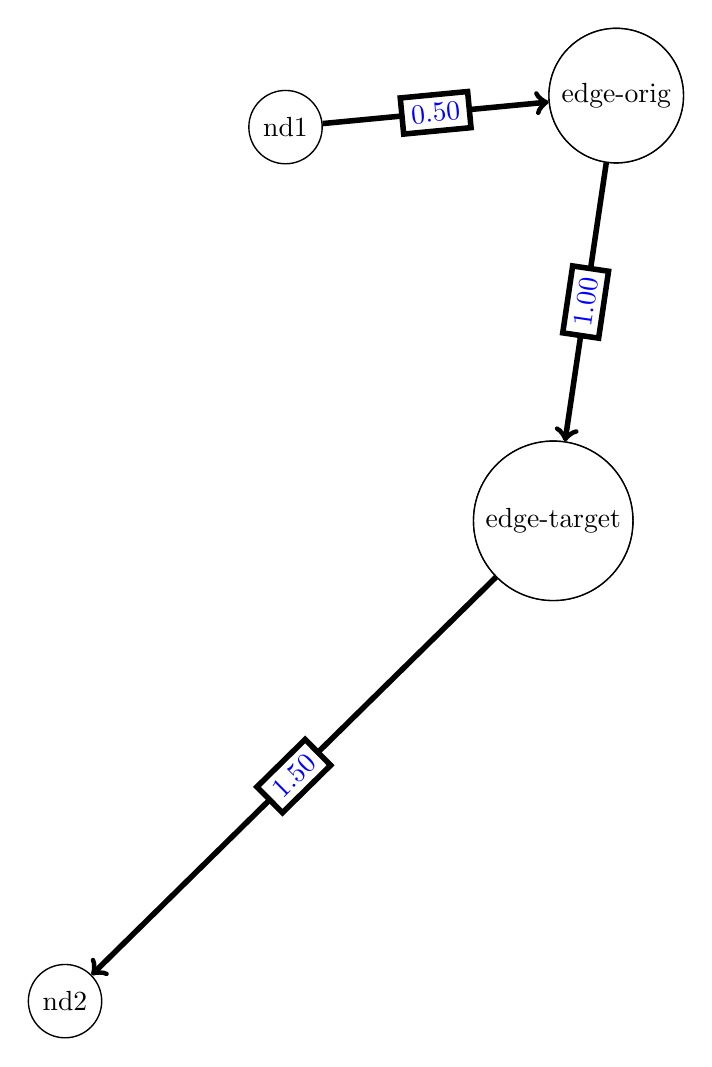
\begin{tikzpicture}
                \SetVertexNormal[Shape      = circle, FillColor  = orange, LineWidth  = 2pt]
                \SetUpEdge[lw  = 2pt,  color      = black,  labelcolor = white,  labeltext  = red, labelstyle = {sloped,draw,text=blue}]
                \GraphInit[vstyle=Normal]
                \SetGraphUnit{10}

                
 
                
                \tikzset{VertexStyle/.append  style={fill}}
                \Vertex[x=6.8 ,y=11.6]{nd1}
          
                
                \tikzset{VertexStyle/.append  style={fill}}
                \Vertex[x=11.0 ,y=12.0]{edge-orig}
          
                \tikzset{EdgeStyle/.style={->}}
                \Edge[label=$0.50$](nd1)(edge-orig)

          

                
                \tikzset{VertexStyle/.append  style={fill}}
                \Vertex[x=11.0 ,y=12.0]{edge-orig}
          
                
                \tikzset{VertexStyle/.append  style={fill}}
                \Vertex[x=10.2 ,y=6.6]{edge-target}
          
                \tikzset{EdgeStyle/.style={->}}
                \Edge[label=$1.00$](edge-orig)(edge-target)

          

                
                \tikzset{VertexStyle/.append  style={fill}}
                \Vertex[x=10.2 ,y=6.6]{edge-target}
          
                
                \tikzset{VertexStyle/.append  style={fill}}
                \Vertex[x=4.0 ,y=0.5]{nd2}
          
                \tikzset{EdgeStyle/.style={->}}
                \Edge[label=$1.50$](edge-target)(nd2)

          


                \end{tikzpicture}

                \mbox{Total weight: 3.000000}

                \end{center}
                \end{document}
          